% Copyright (c) 2016 Ongun Kanat <ongun.kanat@gmail.com>
% This document is a free software licensed under MIT license.
% For redistribution details look at COPYING file.

% 12pt and ISO A4 paper with title page add notitlepage for otherwise
\documentclass[a4paper, 12pt, titlepage]{article}

% 2cm margin from all sides
\usepackage[a4paper,margin=2cm]{geometry}

% Use American English for dates etc.
\usepackage[american]{babel}
% If document is in Turkish then use
% \usepackage[turkish]{babel}
% or for both
% \usepackage[turkish,american]{babel}

% Indent at section beginnings
% \usepackage{indentfirst} % look at below for reverse
% Paragraph spacings set parindent to 0
\setlength{\parindent}{0pt}
\setlength{\parskip}{12pt}

% utf-8 support
\usepackage[utf8]{inputenc}

% Graphics for PDFTeX
\usepackage[pdftex]{graphicx}

% Figure placement
\usepackage{float}

% An enumeration package for flexible enumeration
\usepackage{enumitem}

% Courier monospace font
\usepackage{courier}

% Links, both local and external
\usepackage{hyperref}
\hypersetup{
	unicode=true,
	colorlinks=true,
	urlcolor=blue,
	citecolor=black,
	menucolor=black,
	linkcolor=black
}

% Figure captions are bold
\usepackage[labelfont=bf]{caption}

% Pseudocode
\usepackage{algorithmicx}
\usepackage{algpseudocode}
\usepackage{algorithm}
\MakeRobust{\Call}

%tikz for figures
\usepackage{tikz}
\usepackage{pgfplots}

% Syntax highlighting simple
\usepackage{listings}
\lstset{basicstyle=\ttfamily,frame=lines,tabsize=4}
\renewcommand{\lstlistingname}{Code}

% Syntax higlighting (advanced)
%\usepackage{minted}

% Title, author and date info
\title{BLG 335E Analysis of Algorithms I - Assignment II Report}
\author{Mehmet Eymen Ünay \\ 040190218}
\date{December 2, 2022}

\begin{document}
% Fix Turkish fix hypenation
%\shorthandoff{=}

% For a generic title page one can use standard \maketitle command
% It will use the title info above
% \maketitle

% The title page can be made by hand as below
\begin{titlepage}
	\begin{center}
		\large{Istanbul Technical University \\ Faculty of Computer and Informatics \\ Computer Engineering Department} \\
		\vspace{150pt}
		\Large{BLG 335E Analysis of Algorithms I - Assignment II Report}  \\
		\vspace{30pt}

		\large{Mehmet Eymen Ünay \\ 040190218} \\
		\vspace{\fill} % Fill out until the page end
		\large{December 2\textsuperscript{nd}, 2022}
	\end{center}
\end{titlepage}
\pagenumbering{roman}
\newpage
\tableofcontents
\newpage

% For the ones who doesn't know: 1,2,..9 called West Arabic numbers
\pagenumbering{arabic}
\section{Introduction}
The assignment's requirement is to process a stream of numbers and evaluate statistics. As the assignment states it, an incremental approach to evaluation is embraced rather than analysing the whole input file beforehand. As every statistical feature can be deactivated at the beginning of the input file, modularity at evaluation of each statistical value is preserved. This modularity caused several similar data structures and similar calls to these structures but the ease of maintenance and deactivation ability made me favour a more modular approach. 

\section{Code Internals}
\subsection{Data Structures}
To store which statistical values are desired at output a struct with every value corresponding to a bool is created and checked throughout the code to prevent unnecessary calculations or writes.
\par
Every statistical value and their companions are stored in their corresponding struct in a global data\_structures struct. Additional to their own values, the structs contain companion structures. Std has all the relevant data in a vector which it computes with. Each of median, firstq and thirdq has two heaps, a max and min heap. Quartiles have 3:1 size ratios of heaps and median has 1:1 size ratio. 
\subsection{Functions}
To optimize for performance, costly operations such as sorting is avoided and instead heaps are used to take the load of storing minimum and maximums of regions of interest. Functions about heap are in heap.h.
\par
The worst case recurrence relation of a Max\_heapify function with pseudocode at Algorithm \ref{algo:max_heapify}, is \( T(n) <= T(2n/3) + \Theta(1)\). Using Case 2 of Master Method \(T(n) = O(lg n)\)
\begin{algorithm}[]
	\caption{Max\_heapify}
	\label{algo:max_heapify}
	\begin{algorithmic}
	\State \textbf{Maxheap} $M$
	\Function{Max\_heapify}{$M$, $i$}
        \State $l \gets$ \Call{Left}{$ i $}
        \State $r \gets$ \Call{Right}{$ i $}
        \State $largest \gets$ $i$
        \If{$l$  lte heap\_size and A[$l$] gt A[$i$]) } \Comment if left child is larger make it the largest
		      \State  $ largest \gets$  $l$ 
        \Else
            \State  $ largest \gets$  $i$
        \EndIf
        \If{$r$  lte heap\_size and A[$r$] gt A[$largest$])} \Comment if right child is larger make it the largest
            \State  $ largest \gets$  $r$ 
        \EndIf
        \If{ $largest$ ne $i$} \Comment if one of the childs were larger
            \State \Call{Swap}{A[$ i $], A[$largest$]} \Comment swap largest child with index at parent
            \State \Call{Max\_heapify}{A, $largest$} \Comment recursive call to itself from child
	    \EndIf
	\EndFunction
	\end{algorithmic}
\end{algorithm}

The Algorithm \ref{algo:build_max_heap} provides the ability to build a heap from an unsorted array though it is not used as every heap is built from scratch. Its asymptotic bound is \(O(n)\). 
\begin{algorithm}[]
	\caption{Build\_Max\_Heap}
	\label{algo:build_max_heap}
	\begin{algorithmic}
	\State \textbf{Array} $A$
	\Function{Build\_Max\_Heap}{$A$}
        \State $heap_size \gets$ \Call{Length}{A}
        \ForAll{$i \gets $ \Call{Floor}{\Call{Length}{A}/2} downto 1} \Comment Runs from the parents with children 
            \State \Call{Max\_heapify}{A,$i$}
        \EndFor
	\EndFunction
	\end{algorithmic}
\end{algorithm}

The Algorithm \ref{algo:extract_max_heap} returns the root node and deletes it at the heap. Calls algorithm \ref{algo:max_heapify} to restore the heap property. Its analysis is similar to algorithm \ref{algo:max_heapify} since the remaining code adds constant complexity.

\begin{algorithm}[]
	\caption{Extract\_Max\_Heap}
	\label{algo:extract_max_heap}
	\begin{algorithmic}
	\State \textbf{Heap} $M$
	\Function{Extract\_Max\_Heap}{$A$}
        \State $max \gets$ $M$[1] \Comment Root node
        \State $M[1] \gets$ $M[heap_size]$ \Comment last element becomes the root
        \State $heap_size--$
        \State \Call{Pop\_back}{$M$} \Comment last element deleted
        \State \Call{Max\_Heapify}{$M$, $1$}
        \Return max
	\EndFunction
	\end{algorithmic}
\end{algorithm}

\section{Application of Data Structures}
There are two classes which coordinate and operate on the required inputs: Stats class which has the calculate functions and Manager class which coordinates when to call calculate and adds new data to the corresponding data structures.
\par
When new data arrives add\_element function of Manager runs and checks which options are set. Accordingly, runs calculate functions of mean std, renews min and max, adds data to std's vector and adds elements to heaps of order statistical values. After adding data to vector and heaps their corresponding statistical calculation functions at Stats are called.
\par
Double heap structures for order statistics is used. To implement median, two cases are checked. If sizes of heaps are equal, new element is added to max heap and the heap gets sifted which updates the min heap. The case for different size is similar with the direction in reverse. To calculate median sizes are checked and returned from max or interpolated accordingly.
\par
Achieving similar structure at quartiles requires 4 states to check but is similar to median in essence. The calculate function uses Gumbel quartile interpolation according to new states after the element is added.

\section{Performance Analysis}
To minimise the effects of standard deviation and mean calculations, Welford's online algorithm is used. Compared to naive implementation, it reduced the growth complexity close to  \(O(logn)\) as it can be estimated from the plot below referring heap based order calculation complexities. 

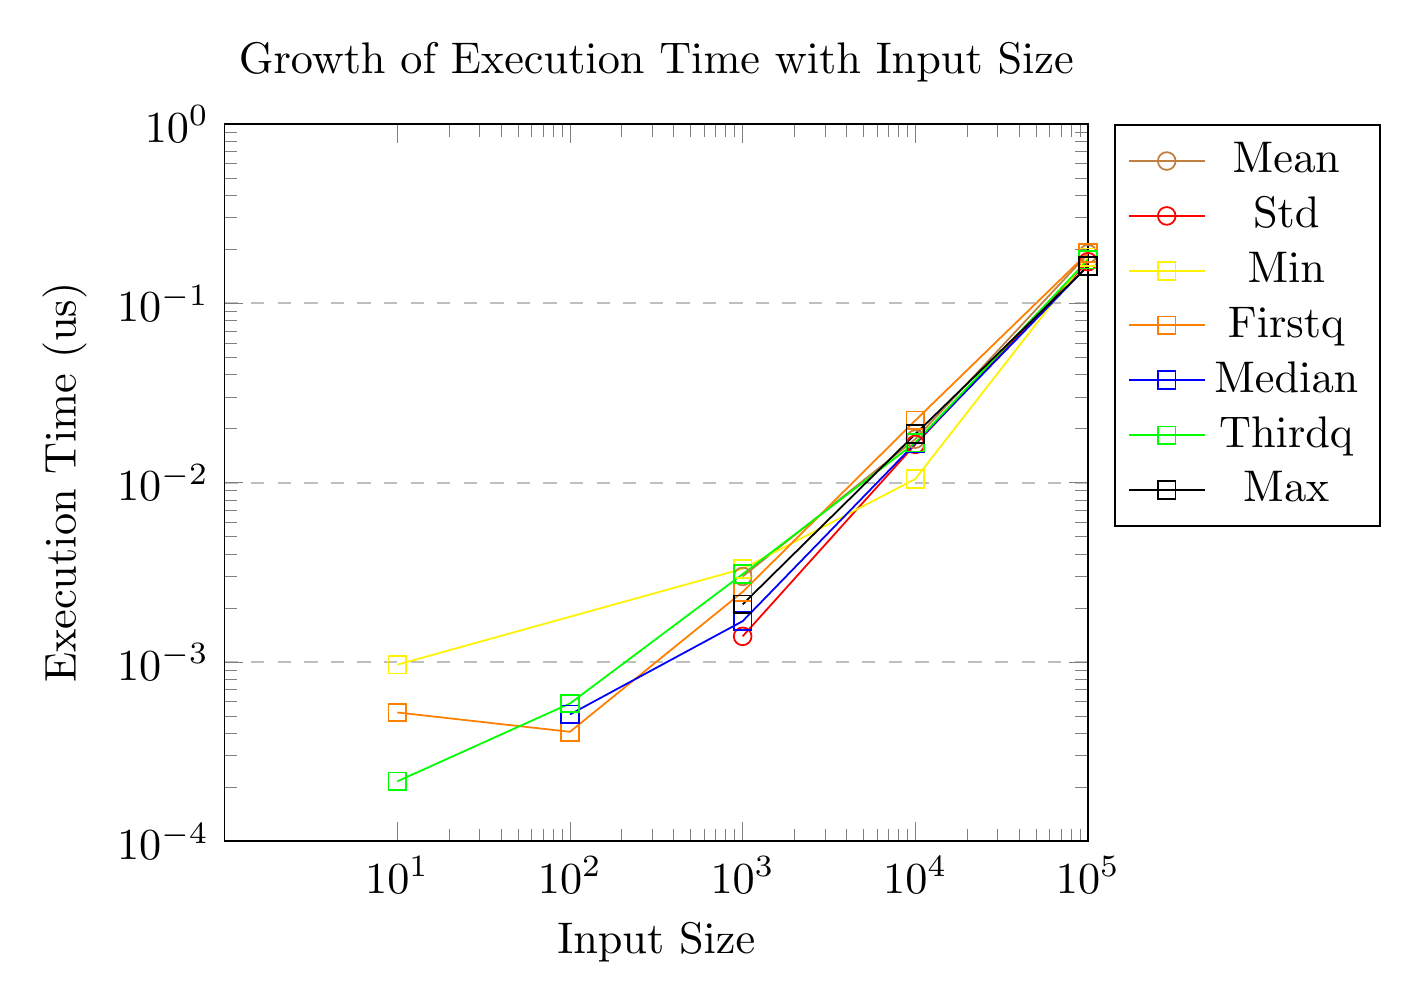
\begin{tikzpicture}[scale=1.6]
\begin{axis}[
    xmode=log,
    ymode=log,
        title={Growth of Execution Time with Input Size},
    xlabel={Input Size},
    ylabel={Execution Time (us) },
    xmin=1, xmax=100000,
    ymin=0.0001, ymax=1,
    xtick={10,100,1000,10000, 100000},
    ytick={0.0001,0.001,0.01,0.1,1},
    legend pos= outer north east,
    ymajorgrids=true,
    grid style=dashed
]
%mean
\addplot[ 
    color=brown,
    mark=o,
    ]
    coordinates {
    (10,0)(100,0)(1000,0.002999)(10000,0.017488)(100000,0.189016)
    };
%std
\addplot[ 
    color=red,
    mark=o,
    ]
    coordinates {
    (10,0)(100,0)(1000,0.001390)(10000,0.016340)(100000,0.170660)

    };
%min
\addplot[ 
    color=yellow,
    mark=square,
    ]
    coordinates {
(10,0.000966)(100,0)(1000,0.003309)(10000,0.010486)(100000,0.180308)    };
%firstq
\addplot[
    color=orange,
    mark=square,
    ]
    coordinates {
(10,0.000523)(100,0.000408)(1000,0.002460)(10000,0.022239)(100000,0.191322)    };
%median
\addplot[ 
    color=blue,
    mark=square,
    ]
    coordinates {
(10,0)(100,0.000510)(1000,0.001689)(10000,0.016570)(100000,0.162131)    };
 %thirdq
\addplot[  
    color=green,
    mark=square,
    ]
    coordinates {
(10,0.000216)(100,0.000587)(1000,0.003088)(10000,0.016724)(100000,0.175352)    };
 %max
\addplot[  
    color=black,
    mark=square,
    ]
    coordinates {
(10,0)(100,0)(1000,0.002096)(10000,0.018656)(100000,0.161441)    };
    \legend{Mean, Std, Min, Firstq, Median , Thirdq, Max}

\end{axis}
\end{tikzpicture}
\section{Discussion}
Using a sliding window based method is possible since  instead of waiting for the data to arrive and accumulate it, we could move over the data and calculate accordingly. Irrelevant parts of data structures could be pruned which is not possible at a sorting based approach.

Though heaps provided immense speed in finding the quartiles and the median, it seemed redundant to use three pairs of heaps to provide related information about the same data. Though the memory complexity is constantly growing, if the memory would like to be optimised against speed an approach combining all three structures is possible. The structure requires a special type of heap called min-max heap which is a heap slightly more complicated to use but stores both min and max of the data. By using this heap it is possible to find the first quartile, median and third quartile from a single entity. To build the structure it would be needed to have 4 heaps of same size. From the minimum to the first quartile of the data can be stored in a max heap and the data from the maximum of data to its third quartile can be stored in the min heap. For the remaining two heaps it would be needed to use the minmax heap discussed above to use the same heaps for both median and its neighbouring quartile. Some implementation of minmax heap can be found in my heap.h file. The problem with this structure is that the addition of elements and the state protection have to be thought thoroughly. A sift in one heap may trigger the next heap to sift. To sum up, less memory can be used by having a more complicated data structure and management system.



\end{document}
